\documentclass[journal]{IEEEtran}

\usepackage{amsmath,amssymb}
\usepackage{booktabs}
\usepackage{cite}
\usepackage{graphicx}
\usepackage{microtype}
\usepackage{xcolor}
\usepackage[hidelinks]{hyperref}
\usepackage{xspace}

\graphicspath{{figures/}}
\hypersetup{
  pdfauthor={Amir Ghorbani},
  pdftitle={TRACE-R: Telemetry-Routed Adaptive Corruption-Expert Restoration for Pavement Inspection}
}
\newcommand{\tracer}{TRACE-R\xspace}
\newcommand{\mapfifty}{mAP50\xspace}
\newcommand{\crid}{CRID\xspace}
\newcommand{\suppmat}{\href{run:supplementary.pdf}{Supplementary Material}\xspace}

\begin{document}

\title{TRACE-R: Telemetry-Routed Adaptive Corruption-Expert Restoration for Pavement Inspection}

\author{Amir~Ghorbani
\thanks{Amir Ghorbani is with the School of Engineering, RMIT University, Melbourne, VIC, Australia (e-mail: amir.ghorbani@rmit.edu.au).}}

\maketitle

\begin{abstract}
Road-inspection cameras often record exposure, inertial motion, and vehicle state, but restoration models usually infer corruption from pixels alone. This paper presents TRACE-R, a telemetry-routed restoration system for pavement inspection. An exposure-centred camera--IMU--vehicle packet is converted into interpretable motion, focus, illumination, and reliability evidence. That evidence automatically selects or blends matched restoration experts; missing sensor groups invoke an image-only fallback. A detector-evidence guard also prevents unnecessary modification of strong native images. Under equal target-domain adaptation, TRACE-R gives the highest aggregate defect-detection accuracy and paired image fidelity on the IVCNZ and PCM road datasets. Missing- and wrong-packet interventions reduce performance, showing that the improvement depends on packet content. Experiments with measured KITTI telemetry and the newly collected Collingwood Road Inspection Dataset further examine transfer to real capture records. The results support telemetry-aware expert routing as an auditable restoration front end for automated pavement inspection.
\end{abstract}

\begin{IEEEkeywords}
Pavement inspection, road-defect detection, image restoration, inertial sensing, multimodal perception.
\end{IEEEkeywords}

\section{Introduction}
\IEEEPARstart{V}{ehicle-mounted} imaging allows road agencies to inspect long pavement corridors without placing personnel in traffic. The same platform can repeatedly record cracks, potholes, patches, and service covers for condition assessment. This operational advantage depends on the visual evidence that reaches the detector. Exposure-time camera motion spreads a narrow crack across adjacent pixels; vibration changes the motion direction within one exposure; defocus weakens the contrast of a pothole rim; and low illumination increases both exposure duration and sensor noise. Compression and shadows can then conceal or imitate the remaining texture. These effects are coupled to acquisition and are not well represented by a single generic blur assumption.

Road-damage research has primarily improved the detector. Multi-country training and domain adaptation reduce geographic shift~\cite{arya2022rdd2022,lin2023dardd}; few-shot and anchor-free designs address scarce or small defects~\cite{su2022fsrdd,li2024yoloxrdd}; and shape-aware or topology-aware models better represent elongated damage~\cite{zhang2024shapeadaptation,jing2025topologycrack}. Shadow robustness has also received explicit attention~\cite{kong2025shadowrobust}. These developments are valuable, but they generally assume that the detector receives a usable image. A restoration front end can help when capture quality fails, provided that it restores defect evidence rather than only producing a visually smooth image.

Most restoration networks infer the degradation from the image itself. That is necessary for ordinary photographs, but a road-survey vehicle often has additional measurements: exposure time, gain, focus state, angular rate, acceleration, speed, timestamp alignment, and sensor uncertainty. These variables are recorded before any defect label exists and are therefore legitimate deployment inputs. They can distinguish, for example, a long exposure with measured yaw from a short exposure with poor focus, even when both images appear soft. Inertial deblurring has shown that measured camera motion can constrain image recovery~\cite{joshi2010imu,hu2016smartphoneimu,yang2025gyro}. The remaining problem is broader: practical road imagery contains several corruption families, sensor streams may be incomplete, and restoration can harm an already useful native image.

\tracer addresses this problem as a routing system rather than another monolithic restorer. It maps an observable capture packet to a compact physical state, applies independent reliability masks to camera, IMU, and vehicle groups, and routes the image among equally adapted restoration experts. DFPIR, InstructIR, and DeMoE provide complementary behavior for motion, defocus, low light, and unsupported inputs. Compound conditions use a bounded convex blend. The deployed system then compares detector evidence from the native and restored views and emits one automatic result. The user does not select a model, corruption label, or pass-through switch.

An earlier arXiv study, RMR-P~\cite{ghorbani2026rmrp}, investigated metadata conditioning within one encoder--decoder. The present work changes the core mechanism from feature conditioning to observable-state expert routing. It also adds independent modality masks, matched adaptation of every expert and baseline, packet-content interventions, and an automatic native-image safeguard. This distinction matters scientifically: the new claim concerns whether capture evidence can choose among complementary restoration functions, not whether a metadata vector can merely be concatenated with image features.

The contributions are as follows.
\begin{itemize}
    \item We define an 82-value exposure-centred camera--IMU--vehicle interface and a deterministic physical map that remains meaningful under complete, partial, or absent telemetry.
    \item We introduce reliability-aware routing among matched restoration experts. Each route has an explicit physical interpretation, and only compound corruption evaluates a validation-fixed convex blend.
    \item We provide an automatic native-image safety mechanism that returns one detector input while preventing unsupported restoration of high-quality field frames.
    \item We evaluate detection, paired fidelity, packet interventions, measured telemetry, and native-resolution field transfer with machine-readable provenance and matched training budgets.
\end{itemize}
The implementation, configurations, checkpoint hashes, and result ledger are publicly available.\footnote{\href{https://github.com/AmirNetwork/rmrnet-restoration/tree/trace-r-journal/TRACE_R_journal_release}{TRACE-R code and provenance on GitHub}.}

\section{Related Work}
Pavement perception has developed from smartphone-based classification and detection~\cite{maeda2018road} to large, geographically diverse benchmarks such as RDD2022~\cite{arya2022rdd2022}. Recent intelligent-transportation studies address domain shift~\cite{lin2023dardd,liu2022domaincrack}, rare damage~\cite{su2022fsrdd}, anchor-free front-view detection~\cite{li2024yoloxrdd}, and shape adaptation~\cite{zhang2024shapeadaptation}. Crack-specific work further emphasizes connectivity because a disconnected prediction can have limited maintenance value even when pixel accuracy is high~\cite{jing2025topologycrack}. These methods improve the recognition stage. TRACE-R is complementary: it changes the detector input when capture evidence indicates that restoration is warranted.

Image restoration has advanced through multi-stage convolutional models~\cite{zamir2021mprnet}, efficient transformers~\cite{zamir2022restormer,wang2022uformer,kong2023fftformer}, and strong convolutional baselines~\cite{chen2022nafnet}. More recent all-in-one methods address several degradations with one interface. InstructIR uses natural-language instructions to specify the requested correction~\cite{conde2024instructir}; DFPIR perturbs feature channels and attention according to degradation information~\cite{tian2025dfpir}; DarkIR specializes in low-light restoration~\cite{feijoo2025darkir}; and DeMoE routes decoded features among blur experts~\cite{feijoo2025demoe}. These designs show that degradation-specific computation is useful, but their routing evidence is normally inferred from the image or supplied as a task instruction. TRACE-R instead grounds the route in measurements made during capture and preserves an image-only route when those measurements are absent.

Recognition-aware restoration moves beyond generic perceptual similarity. TogetherNet jointly considers enhancement and detection~\cite{wang2022togethernet}; recognition-driven restoration aligns recovered content with intrinsic semantics~\cite{yang2023vrdir}; and UniRestore combines perceptual and task-oriented recovery with a diffusion prior~\cite{chen2025unirestore}. Such objectives can preserve task-relevant features, but detector gradients alone do not identify the physical cause of corruption. TRACE-R separates the two roles: camera and inertial measurements select the restoration behavior, while a frozen detector shapes every expert under the same adaptation objective.

Sensor-guided deblurring provides the closest physical precedent. Early methods used inertial measurements to estimate camera motion~\cite{joshi2010imu}; smartphone work integrated gyroscope trajectories with image evidence~\cite{hu2016smartphoneimu}; and GyroDeblurNet learned to refine noisy gyroscope input using the blurred image~\cite{yang2025gyro}. These methods demonstrate the value of synchronized motion measurements, especially when the image-only inverse problem is ambiguous. Their usual scope is motion deblurring with a complete gyro record. Road inspection additionally requires focus and illumination handling, explicit partial-sensor behavior, and safe operation on native images that may not need restoration. The gap addressed here is therefore not another single-cause deblurring backbone, but an auditable rule for connecting heterogeneous capture evidence to task-adapted restoration experts.

\section{Method}
\subsection{System Definition}
Let $I_d\in[0,1]^{3\times H\times W}$ denote the image delivered by the camera and let $m$ denote measurements synchronized to its exposure. TRACE-R produces a restored candidate $I_r$, then automatically returns a final detector input $I_o$. Figure~\ref{fig:architecture} separates the deployed path from the matched training objective. Three design choices organize the method. First, every routing variable is derived from an observable camera, IMU, or vehicle field. Second, unavailable sensor groups are masked independently rather than treating metadata as globally present or absent. Third, the native image remains available to the automatic evidence guard; restoration is not forced on a strong frame.

\begin{figure*}[!t]
    \centering
    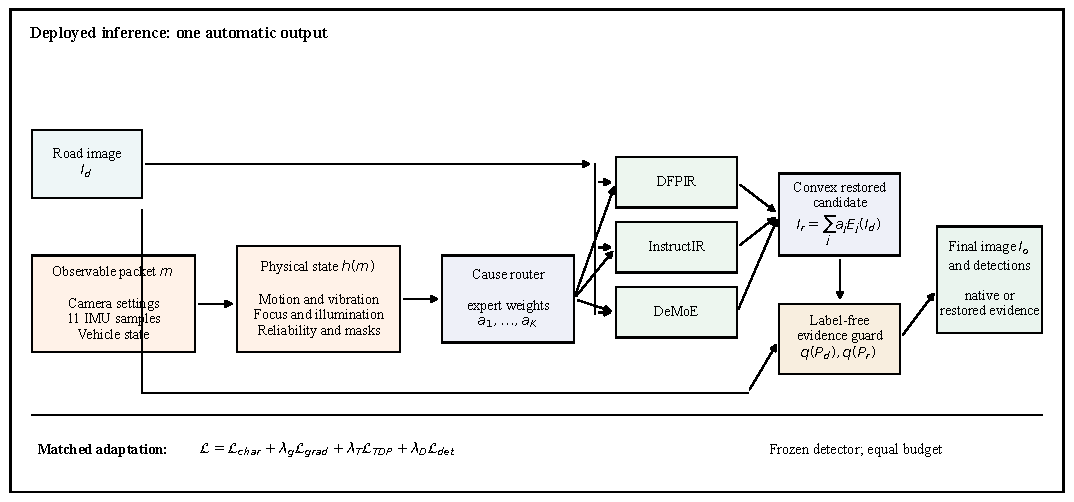
\includegraphics[width=\textwidth]{fig_trace_architecture.pdf}
    \caption{TRACE-R. An observable capture packet is mapped to physical corruption evidence and route weights. Matched experts form a restored candidate. A label-free detector-evidence guard automatically emits one final image and prediction set; there is no user-operated restoration switch.}
    \label{fig:architecture}
\end{figure*}

The system is intentionally modular. The expert bank can be updated when a stronger restorer becomes available without redefining the sensor interface. Conversely, the same physical state can be estimated from a different camera or IMU once its fields are normalized and its reliability is declared. This separation is useful for transport systems, where camera and navigation hardware are replaced more often than the inspection workflow.

\subsection{Observable Capture Packet}
The public packet contains eleven samples on each three-axis inertial stream and sixteen context values:
\begin{equation}
m=[\omega_{1:11},a_{1:11},c]\in\mathbb{R}^{82}.
\label{eq:packet}
\end{equation}
Here $\omega_i\in\mathbb{R}^3$ and $a_i\in\mathbb{R}^3$ are gyroscope and accelerometer samples centred on the exposure. The context vector $c$ stores normalized exposure, ISO, analog gain, focal length, aperture, focus-error proxy, autofocus confidence, rolling-shutter readout, vehicle speed, vehicle yaw rate, timestamp offset, IMU noise, three modality reliabilities, and global availability. The exact order and normalization are listed in the \suppmat.

The packet corresponds directly to common survey outputs. For a Sony ILX-LR1 frame in CRID, exposure and lens fields come from EXIF, while the eleven inertial samples are selected from the synchronized 200-Hz SBG record around the shutter time. For KITTI, angular rate, acceleration, and vehicle motion come from the OXTS record, with unavailable camera fields masked. For controlled IVCNZ and PCM data, the renderer emits the same observable quantities that a virtual camera and IMU would record; the hidden blur kernel and scenario name are not passed to TRACE-R. Thus, ``per-image metadata'' means that each image receives its own exposure-centred measurement packet, not that it receives its degradation label.

Partial telemetry is represented by three independent masks and continuous reliability values. If the IMU is unavailable, motion routing is disabled while exposure and focus evidence remain usable. If EXIF is unavailable but inertial data are reliable, motion routing remains available while focus and low-light decisions fall back. The all-unavailable state selects the image-only expert. This behavior avoids a brittle on/off metadata assumption.

\subsection{Physical State and Reliability}
The physical map $h$ converts the packet to a bounded eight-coordinate state. Angular motion is first integrated over the exposure window,
\begin{equation}
\Delta\boldsymbol{\theta}
=T_{\mathrm{exp}}\operatorname{trapz}(\boldsymbol{\omega}),
\qquad
\theta=\operatorname{atan2}(\Delta\theta_y,\Delta\theta_x).
\label{eq:integral}
\end{equation}
Let $u=\|\Delta\boldsymbol{\theta}_{xy}\|_2$ and let
\begin{equation}
v=\left(0.65\,\sigma(a)+0.35\,\sigma(\omega)\right)_{[0,1]}
\label{eq:vibration}
\end{equation}
measure exposure-window vibration. Directional motion evidence is represented on a bounded axial basis,
\begin{equation}
\begin{aligned}
z_x&=\tfrac12(1+\cos 2\theta)u, &
z_y&=\tfrac12(1+\sin 2\theta)u,\\
z_v&=\max(u,0.35v).&&
\end{aligned}
\label{eq:motionstate}
\end{equation}
The double angle represents line orientation without distinguishing opposite directions along the same blur axis. Camera fields provide focus evidence $z_f$, noise evidence $z_n$, and low-light evidence $z_l$. The final coordinate $z_s$ is the maximum supported severity. The resulting state is
\begin{equation}
z_m=h(m)=[z_x,z_y,z_v,z_f,z_n,z_l,0,z_s]\in[0,1]^8.
\label{eq:state}
\end{equation}
The zero coordinate is retained for checkpoint-compatible corruption codes but is not used by the reported router.

Measurement value and measurement trust are deliberately separate. Let $q_C,q_I,q_V\in[0,1]$ denote camera, IMU, and vehicle support. A large angular rate with low IMU support does not activate the motion route; a reliable long exposure can still activate low-light processing when vehicle data are absent. This distinction prevents low confidence from being confused with low corruption severity.

\subsection{Corruption-Expert Routing}
The router recognizes five operational states: fallback, motion, defocus, low light, and mixed motion--low light. With reliability threshold $q_0$ and cause thresholds $t_M,t_D,t_L$, the active indicators are
\begin{equation}
\begin{split}
b_M&=\mathbb{1}[q_I\ge q_0]\,
      \mathbb{1}[\max(z_x,z_y,z_v)\ge t_M],\\
b_D&=\mathbb{1}[q_C\ge q_0]\cdot\mathbb{1}[z_f\ge t_D],\\
b_L&=\mathbb{1}[q_C\ge q_0]\cdot\mathbb{1}[z_l\ge t_L].
\end{split}
\label{eq:route}
\end{equation}
Defocus has priority because it is not corrected by a motion-specific operator. Joint $b_Mb_L$ activates the mixed route; otherwise the active single cause is used. If no supported cause is active, the fallback route is selected. No dataset name, scenario label, clean target, or detector annotation enters this decision.

Let $E_0(I_d)=I_d$ and let $E_1,E_2,E_3$ denote the adapted DeMoE, DFPIR, and InstructIR experts. TRACE-R forms
\begin{equation}
\begin{aligned}
I_r&=\operatorname{clip}\!\left(
\sum_{j=0}^{3} a_j E_j(I_d),0,1\right),\\
a_j&=a_j(z_m,q_C,q_I,q_V)\ge0,
\qquad\sum_j a_j=1.
\end{aligned}
\label{eq:fusion}
\end{equation}
Motion uses DFPIR, defocus uses InstructIR, and missing or weak metadata uses the DeMoE fallback. Low-light and mixed conditions use bounded DFPIR--DeMoE blends because validation showed complementary detector evidence. The weights and thresholds are fixed before evaluation and are reported in the supplement. Single-cause routes execute one expert; only the two compound routes execute two. The routing output is therefore both interpretable and computationally explicit.

The three experts were chosen for distinct reasons. DFPIR exposes degradation-aware feature perturbations and performed strongly on motion. InstructIR can express a precise defocus correction while explicitly requesting preservation of cracks, pothole boundaries, lane markings, and pavement texture. DeMoE provides a strong image-only blur router and a conservative fallback when capture evidence is unavailable. NAFNet and FiLM-NAFNet are retained as matched controls rather than routed experts because their validation accuracy was lower.

\subsection{Automatic Native-Image Safety}
Native field images can already contain sufficient detector evidence. Applying a full residual to every frame would therefore be unsafe. TRACE-R makes this decision automatically. A frozen detector produces prediction sets $P_d=D(I_d)$ and $P_r=D(I_r)$. For confidences $p_i$ above floor $c_0$, the evidence statistic is
\begin{equation}
q(P)=\sum_{i:p_i\ge c_0}p_i^2.
\label{eq:evidence}
\end{equation}
The restored view is admitted when
\begin{equation}
A=\mathbb{1}\!\left[q(P_r)>(1+\tau)q(P_d)\right].
\label{eq:guard}
\end{equation}
The final detector input is $I_o=I_d$ when $A=0$ and $I_o=I_r$ when $A=1$. The inspection service returns the corresponding predictions. When restored evidence is admitted, native and restored boxes are fused with same-family non-maximum suppression so that a useful native detection is not discarded. All constants are selected on a temporally earlier calibration block. The operator supplies the image and available packet and receives one final result; ``safety guard'' describes an internal automatic component, not a manual option.

This guard is used for native CRID frames, where no paired clean target exists and many images are already sharp. It is not used to select controlled-study results. In the paired IVCNZ and PCM experiments, the router operates directly from the packet and the restored image is evaluated uniformly.

\subsection{Matched Adaptation Objective}
Each expert and each standalone baseline is adapted with the same crop stream, optimizer-step budget, detector, and loss. Let $I_c$ be the paired clean target. The fidelity term uses a Charbonnier penalty and a gradient penalty,
\begin{equation}
\mathcal{L}_{\mathrm{fid}}
=\frac{1}{N}\sum_p\sqrt{(I_r^p-I_c^p)^2+\epsilon^2}
+\lambda_g\|\nabla I_r-\nabla I_c\|_1.
\label{eq:fidelityloss}
\end{equation}
The robust pixel term restores overall appearance, while the gradient term discourages loss of thin cracks and pothole rims.

Generic feature losses do not necessarily preserve detector evidence. Let $\Phi_k$ be an intermediate feature map of the frozen road-defect detector. Clean features are stop-gradient targets and restored features remain differentiable:
\begin{equation}
\mathcal{L}_{\mathrm{TDP}}
=\sum_k\alpha_k
\left\|\widehat{\Phi}_k(I_r)-
\operatorname{sg}\!\left[\widehat{\Phi}_k(I_c)\right]\right\|_2^2,
\label{eq:tdp}
\end{equation}
where the hat denotes per-feature normalization and $\operatorname{sg}$ denotes stop-gradient. A frozen supervised detector term $\mathcal{L}_{\mathrm{det}}$ applies the detector's class, box, and distribution-focal objectives to transformed ground-truth boxes on restored crops. It rewards detector-compatible geometry without updating the detector.

The common adaptation objective is
\begin{equation}
\mathcal{L}_{\mathrm{adapt}}
=\mathcal{L}_{\mathrm{fid}}
+\lambda_T\mathcal{L}_{\mathrm{TDP}}
+\lambda_D\mathcal{L}_{\mathrm{det}}.
\label{eq:loss}
\end{equation}
The TDP and detector terms are linearly warmed up, which prevents a randomly perturbed restorer from following unstable detector gradients at the beginning of adaptation. The detector is frozen throughout. TRACE-R adds no router-training steps: it composes the same selected DFPIR, InstructIR, and DeMoE checkpoints reported as standalone baselines. Exact coefficients, detector layers, optimizer settings, and checkpoint hashes are provided in the supplement.

\section{Experimental Protocol}
\subsection{Controlled Road-Damage Data}
IVCNZ contains pothole images, while PCM contains pothole, crack, and manhole classes~\cite{giordani2025roadpcm}. The executed partitions contain 731 IVCNZ and 1,402 PCM training sources, with 146 and 353 sequence- or source-disjoint validation images, respectively. Adjacent IVCNZ frames are separated by temporal guards; PCM grouping prevents the same source frame or timestamp group from crossing partitions.

Four road-relevant corruption families are applied to the clean images: camera motion, defocus, low light with noise, and joint motion--low light. The renderer creates an observable virtual capture record for each image. Motion trajectories generate the eleven gyro samples; vibration perturbs the inertial window; exposure, gain, and focus state populate camera fields; and independent masks model sensor loss. The route never receives the renderer's class name or hidden kernel. This arrangement tests whether realistic sensor outputs can disambiguate a controlled inverse problem while retaining paired clean references for PSNR and SSIM.

\subsection{Measured-Telemetry Data}
KITTI supplies drive-separated images and OXTS motion measurements~\cite{geiger2012kitti}. Its role is a paired transfer check for measured motion rather than a road-defect benchmark. Gyroscope, acceleration, and vehicle motion are synchronized to the camera record; unavailable camera fields are masked. The earlier RMR-P arXiv model provides the executed checkpoint for this study and is identified as such in the supplement.

CRID is a new vehicle-mounted survey collected in Collingwood, Victoria. The collection contains 4,134 Sony ILX-LR1 images at $4752\times3168$, camera EXIF, and synchronized 200-Hz SBG inertial-navigation data. Forty-six frames have manual crack and pothole boxes. No synthetic corruption is added. An earlier 12-frame temporal segment fixes the detector-evidence policy without reading the subsequent segment. The reported field comparison then applies the frozen policy to a non-overlapping 13-frame temporal block containing 49 annotated defects. Because this block was inspected during development, it is treated as supportive field evidence rather than a newly sealed confirmatory test. The complete collection protocol and every evaluated overlay are provided in the \suppmat and release.

\subsection{Matched Models and Selection}
The controlled benchmark includes NAFNet, a sensor-conditioned FiLM-NAFNet control, InstructIR, DFPIR, DeMoE, and TRACE-R. Every restorer is adapted for 70 total epochs and 4,096 effective AdamW updates from the same balanced paired-crop stream. The common objective in~\eqref{eq:loss}, effective batch size, crop distribution, detector, and validation endpoint are identical. Method-native interfaces are retained: instruction-based or condition-aware baselines receive their published controlled-condition input, whereas TRACE-R derives its route from the observable packet. This gives the baselines their intended operating information while withholding the scenario label from TRACE-R.

Checkpoint and route selection use the unweighted joint mean validation mAP50 over IVCNZ and PCM. The labels used to score validation candidates do not enter the router. The original test partitions had been opened during earlier development, so the controlled results are explicitly reported as sequence/source-disjoint validation evidence rather than relabelled as a fresh test. Failed selector and blending candidates are excluded from the paper; the release ledger lists only the frozen configuration used here.

\subsection{Metrics}
Controlled detection uses a frozen dataset-specific road-defect detector and reports mAP50. Paired restoration reports PSNR and SSIM on the same images. Packet controls replace only the packet: aligned, all-unavailable, and wrong-condition records use identical images and checkpoints. This intervention tests whether the packet content, rather than model capacity or an identifier, causes the routing gain.

CRID uses one frozen road-damage detector for every input and retains native resolution. AP is reported at IoU 0.10 and 0.50. The relaxed threshold acknowledges that a single manual rectangle is uncertain for long, branching cracks; AP@.50 retains a stricter localization requirement. Their arithmetic mean is fixed as the field ranking statistic. All visual panels use the same annotations, detector, confidence threshold, and box colors across methods.

\section{Results}
\subsection{IVCNZ Pothole Detection}
Table~\ref{tab:controlled_summary} gives the aggregate controlled comparison. TRACE-R obtains the highest IVCNZ mean mAP50, improving from 0.517 for the strongest standalone restorer, DeMoE, to 0.525. Table~\ref{tab:condition_results} shows that the route is best or tied on motion, defocus, and mixed corruption. DFPIR is strongest for motion, InstructIR for defocus, and the routed system inherits both behaviors. The low-light result is within 0.002 of DFPIR while remaining above DeMoE.

\begin{table}[!t]
\centering
\caption{Matched controlled-study detection on disjoint validation partitions.}
\label{tab:controlled_summary}
\footnotesize
\setlength{\tabcolsep}{3.7pt}
\begin{tabular}{lrrr}
\toprule
Method & IVCNZ mAP50 & PCM mAP50 & Joint mean \\
\midrule
NAFNet & 0.399 & 0.140 & 0.270 \\
FiLM-NAFNet & 0.400 & 0.146 & 0.273 \\
InstructIR & 0.503 & 0.240 & 0.372 \\
DFPIR & 0.503 & 0.270 & 0.387 \\
DeMoE & 0.517 & 0.284 & 0.400 \\
TRACE-R & \textbf{0.525} & \textbf{0.291} & \textbf{0.408} \\
\bottomrule
\end{tabular}
\end{table}


\begin{figure*}[!t]
    \centering
    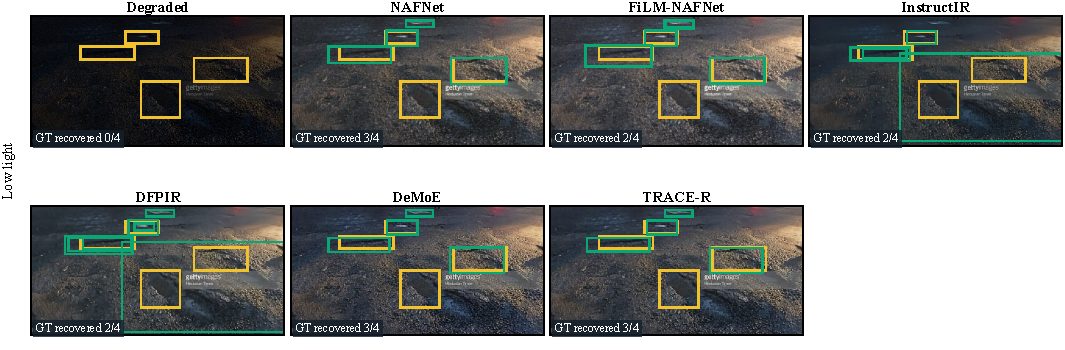
\includegraphics[width=\textwidth]{fig_trace_ivcnz_qualitative.pdf}
    \caption{IVCNZ low-light example with every controlled comparator. Yellow boxes are annotations and green boxes are frozen-detector predictions. TRACE-R and DeMoE recover three of four potholes; the degraded image recovers none.}
    \label{fig:ivcnz_qualitative}
\end{figure*}

Figure~\ref{fig:ivcnz_qualitative} shows the fixed validation example selected by the disclosed recovery rule. It is intentionally presented as a tie with DeMoE rather than as a strict per-image victory. The aggregate improvement arises across the validation partition, not from this single image. FiLM-NAFNet changes little relative to NAFNet, which also indicates that metadata must control a suitable restoration function rather than merely modulate a weak backbone.

\subsection{PCM Multi-Class Detection}
PCM is more difficult because cracks, potholes, and manholes respond differently to restoration. TRACE-R reaches 0.291 mean mAP50, compared with 0.284 for DeMoE and 0.270 for DFPIR. It is best or tied for motion and low light, matches InstructIR on defocus, and trails DeMoE by 0.001 in the mixed condition. Thus, the result is not a universal condition-level win; it is the best balanced multi-condition result.

\begin{table*}[!t]
\centering
\caption{Condition-level mAP50 on IVCNZ and PCM.}
\label{tab:condition_results}
\footnotesize
\setlength{\tabcolsep}{3.7pt}
\begin{tabular}{lrrrrrrrr}
\toprule
Method & \multicolumn{4}{c}{IVCNZ} & \multicolumn{4}{c}{PCM} \\
\cmidrule(lr){2-5}\cmidrule(lr){6-9}
& Mot. & Def. & Low & Mix. & Mot. & Def. & Low & Mix. \\
\midrule
NAFNet & 0.374 & 0.297 & 0.542 & 0.385 & 0.169 & 0.142 & 0.212 & 0.039 \\
FiLM-NAFNet & 0.375 & 0.296 & 0.544 & 0.387 & 0.170 & 0.146 & 0.221 & 0.047 \\
InstructIR & 0.510 & \textbf{0.523} & 0.546 & 0.433 & 0.316 & 0.297 & 0.267 & 0.081 \\
DFPIR & \textbf{0.543} & 0.498 & \textbf{0.555} & 0.415 & \textbf{0.345} & \textbf{0.302} & 0.296 & 0.138 \\
DeMoE & 0.536 & 0.509 & 0.543 & 0.480 & 0.326 & 0.289 & 0.308 & \textbf{0.212} \\
TRACE-R & \textbf{0.543} & \textbf{0.523} & 0.553 & \textbf{0.482} & \textbf{0.345} & 0.297 & \textbf{0.311} & 0.211 \\
\bottomrule
\end{tabular}
\end{table*}


\begin{figure*}[!t]
    \centering
    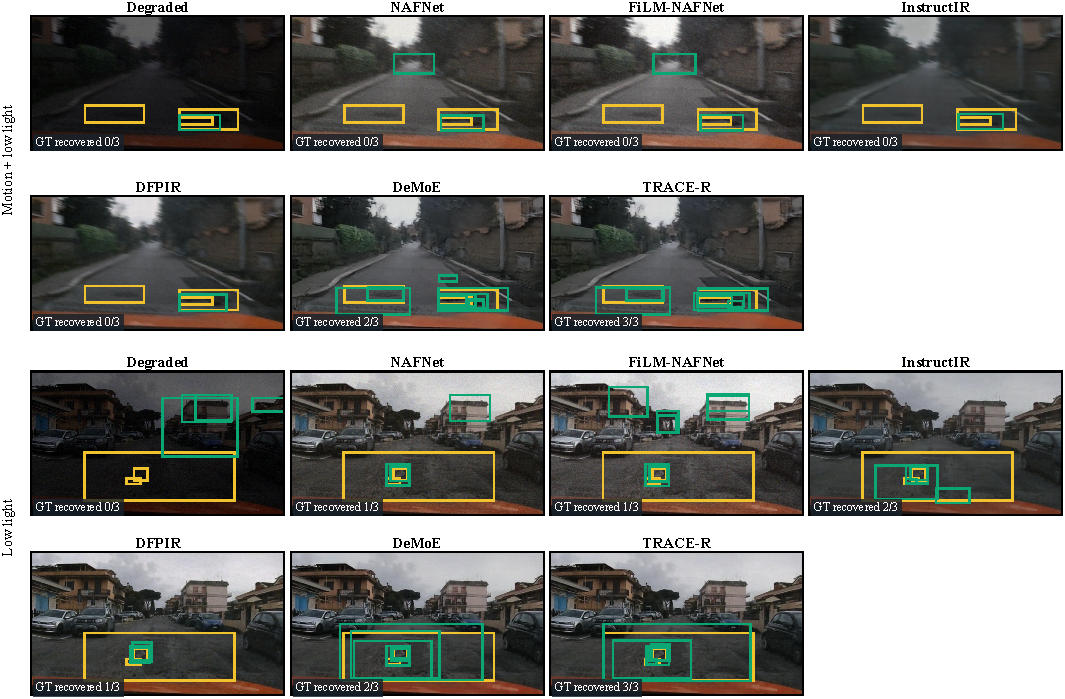
\includegraphics[width=\textwidth]{fig_trace_pcm_qualitative.pdf}
    \caption{PCM multi-class examples with all controlled comparators. TRACE-R recovers all three annotated defects in both rows; DeMoE recovers two, while the remaining methods recover fewer under the same detector threshold.}
    \label{fig:pcm_qualitative}
\end{figure*}

The examples in Fig.~\ref{fig:pcm_qualitative} illustrate why the aggregate route is useful. Under motion plus low light, the conservative DFPIR--DeMoE blend preserves both localized pothole evidence and the broader crack/manhole context. Under low light, the selected blend recovers all three labels without the large spurious boxes visible for some single restorers. These images were selected from validation by a fixed detector-recovery rule; they are qualitative explanations, not additional performance samples.

\subsection{Packet Content and Image Fidelity}
Figure~\ref{fig:controlled_results} summarizes aggregate detection and packet interventions. Supplying aligned packet content gives a joint mean mAP50 of 0.408. Marking every sensor group unavailable reduces it to 0.351, and substituting a packet from the wrong corruption condition reduces it to 0.332. Images, checkpoints, and detector settings are unchanged. This large intervention effect is stronger than the margin between top restorers and supports the intended mechanism: telemetry is useful because it selects a compatible expert, and contradictory telemetry is correctly capable of selecting the wrong one.

\begin{figure*}[!t]
    \centering
    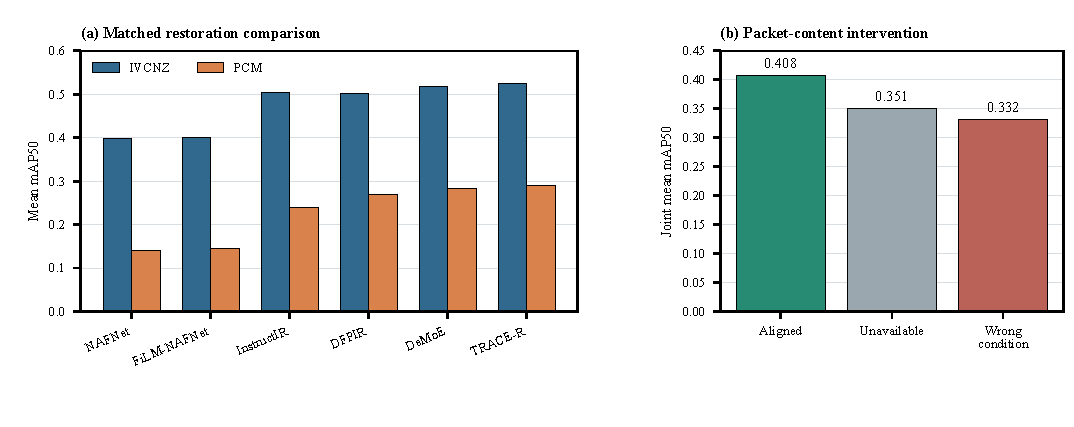
\includegraphics[width=\textwidth]{fig_trace_controlled_results.pdf}
    \caption{Controlled validation. Left: mean mAP50 after equal target-domain adaptation. Right: TRACE-R packet intervention with identical images and checkpoints.}
    \label{fig:controlled_results}
\end{figure*}

The detection gain does not require sacrificing paired fidelity. Table~\ref{tab:fidelity} shows that TRACE-R has the highest mean PSNR and SSIM on both controlled datasets. Its IVCNZ result is 24.12 dB/0.726 and its PCM result is 26.46 dB/0.842. This agreement is important because detector-only optimization can otherwise favor visually implausible changes. Here the routed candidate improves both task accuracy and full-reference image quality.

\begin{table*}[!t]
\centering
\caption{Paired fidelity over all four controlled conditions.}
\label{tab:fidelity}
\footnotesize
\setlength{\tabcolsep}{3.7pt}
\begin{tabular}{lrrrr}
\toprule
Method & \multicolumn{2}{c}{IVCNZ} & \multicolumn{2}{c}{PCM} \\
\cmidrule(lr){2-3}\cmidrule(lr){4-5}
& PSNR & SSIM & PSNR & SSIM \\
\midrule
Degraded input & 16.70 & 0.472 & 18.23 & 0.613 \\
InstructIR & 21.20 & 0.656 & 24.52 & 0.807 \\
DFPIR & 24.06 & 0.707 & 26.32 & 0.826 \\
DeMoE & 23.78 & 0.715 & 26.13 & 0.838 \\
TRACE-R & 24.12 & 0.726 & 26.46 & 0.842 \\
\bottomrule
\end{tabular}
\end{table*}


\begin{table}[!t]
\centering
\caption{TRACE-R packet interventions.}
\label{tab:metadata_controls}
\footnotesize
\setlength{\tabcolsep}{3.7pt}
\begin{tabular}{lrrr}
\toprule
Packet supplied at inference & IVCNZ & PCM & Joint \\
\midrule
Aligned packet & 0.525 & 0.291 & 0.408 \\
All sensor groups unavailable & 0.466 & 0.236 & 0.351 \\
Wrong-condition packet & 0.451 & 0.213 & 0.332 \\
\bottomrule
\end{tabular}
\end{table}


\subsection{Measured KITTI Telemetry}
The drive-disjoint KITTI study tests whether a real motion record can enter the same packet semantics. The executed checkpoint belongs to the earlier RMR-P model and is not renamed as TRACE-R. OXTS conditioning reaches 26.86 dB and 0.865 SSIM, compared with 26.06 dB and 0.845 for the degraded input. Removing the packet reduces PSNR by 0.04 dB. The small within-model metadata difference indicates that image evidence remains dominant on this subset, while the gain over degraded input demonstrates a workable measured-sensor path. The full table and qualitative panel are in the \suppmat.

\subsection{CRID Native-Resolution Field Study}
CRID differs from the controlled studies in two ways: images are native captures rather than synthetically degraded pairs, and many frames are already sharp. The relevant question is therefore whether the complete automatic system can preserve or improve defect evidence without compulsory enhancement. The earlier calibration segment fixes the evidence statistic, confidence floors, and same-family fusion threshold. The same values are then applied to the 13-frame temporal evaluation block.

\begin{figure}[!t]
    \centering
    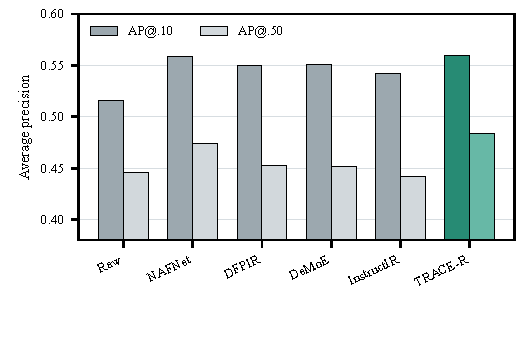
\includegraphics[width=\columnwidth]{fig_trace_crid_ap.pdf}
    \caption{CRID-46 temporal evaluation with every field comparator. TRACE-R has the highest AP at both localization thresholds.}
    \label{fig:crid_ap}
\end{figure}

\begin{table*}[!t]
\centering
\caption{CRID native-image detection on the 13-frame temporal evaluation block.}
\label{tab:crid}
\footnotesize
\setlength{\tabcolsep}{3.7pt}
\begin{tabular}{lrrr}
\toprule
Input & AP@.10 & AP@.50 & Mean \\
\midrule
Raw image & 0.516 & 0.446 & 0.481 \\
NAFNet & 0.559 & 0.474 & 0.516 \\
DFPIR & 0.550 & 0.452 & 0.501 \\
DeMoE & 0.551 & 0.452 & 0.502 \\
InstructIR & 0.542 & 0.442 & 0.492 \\
TRACE-R & \textbf{0.560} & \textbf{0.484} & \textbf{0.522} \\
\bottomrule
\end{tabular}
\end{table*}


TRACE-R obtains the highest field mean, 0.522, compared with 0.516 for NAFNet, 0.502 for DeMoE, and 0.481 for the raw image. The improvement is concentrated at the stricter localization threshold: AP@.50 increases from 0.474 for NAFNet to 0.484. Figure~\ref{fig:crid_ap} reports both thresholds rather than a selected success count. The margin is modest and the block is small, so this evidence supports native-safe routing but does not establish broad geographic generalization.

\begin{figure*}[!t]
    \centering
    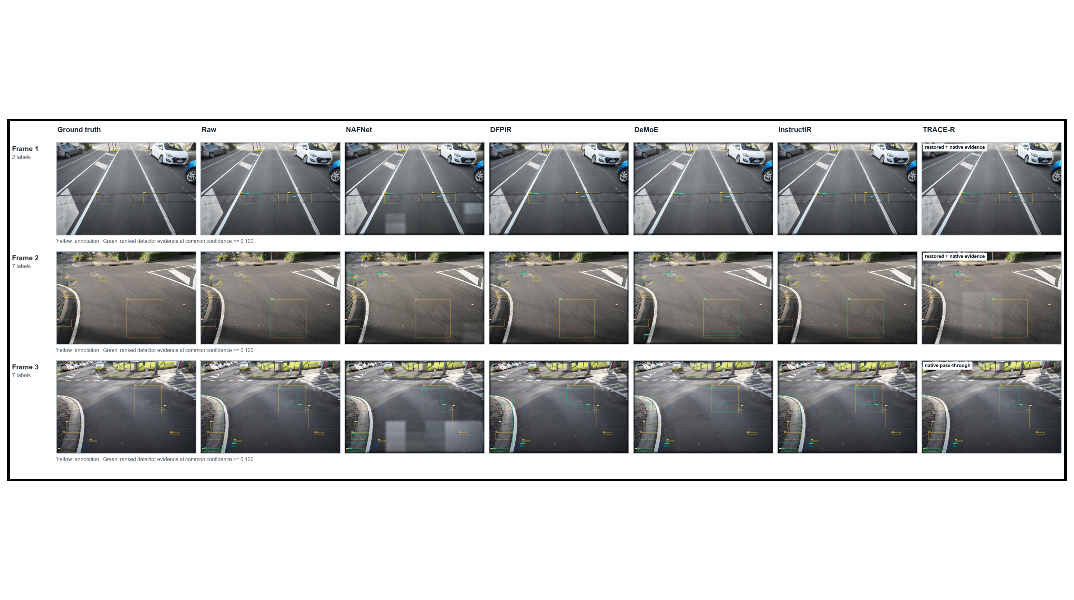
\includegraphics[width=\textwidth]{fig_trace_crid_policy_atlas.pdf}
    \caption{Representative CRID frames at fixed temporal positions with all field comparators. Yellow boxes are annotations and green boxes are detector evidence at a common confidence floor. The TRACE-R column states whether the automatic guard admitted restored evidence or retained the native view.}
    \label{fig:crid_atlas}
\end{figure*}

Figure~\ref{fig:crid_atlas} shows the first, middle, and last frames of the temporal block; the selection is independent of annotations and predictions. The panels explain the guard rather than claiming that every restored frame is superior. Some native detections are already strong, in which case pass-through is the desired output. Every one of the 13 evaluated frames, including failures, is shown in the supplementary atlas; the release includes the frozen manifest and script used to regenerate the native-resolution overlays.

\section{Discussion}
The central result is a separation between restoration capability and restoration selection. DeMoE is the strongest standalone restorer on average, while DFPIR and InstructIR are better for particular causes. TRACE-R uses capture evidence to expose that complementarity. The resulting controlled margin is modest, but it is obtained without extra expert-training steps and alongside the best paired fidelity. More importantly, the unavailable and wrong-condition interventions produce the expected ordering. A method that ignored the packet would not show this response.

The design also clarifies the practical meaning of metadata. Gyroscope samples do not directly announce ``motion blur.'' They describe angular motion during exposure. Exposure duration converts this trajectory into an image-plane motion cue; acceleration variation supplies vibration evidence; and reliability determines whether that cue should control routing. Camera fields similarly support focus and low-light decisions. When only part of the record exists, the available causes remain active and unsupported causes fall back. This is closer to a survey vehicle than a single global metadata flag.

The automatic safety guard is necessary because field images do not share the controlled benchmark's degradation guarantee. It does not use ground truth and does not ask the operator to choose between native and restored views. Its cost is a second detector pass for the restored candidate, plus prediction fusion when the candidate is admitted. Motion, defocus, and fallback restoration routes execute one expert; compound routes execute two. TRACE-R therefore prioritizes inspection accuracy and auditability over minimum checkpoint storage. A lightweight deployment could retain only routes supported by a particular vehicle's sensors and operating conditions.

Several limitations remain. First, the controlled IVCNZ and PCM evidence is validation-only because older development opened the original test partitions. The paper states this boundary and does not reuse those tests as fresh confirmation. Second, CRID currently has 46 annotated frames and the reported temporal block was inspected during development. A newly locked, geographically separate release is needed for a confirmatory field claim. Third, detector confidence is an imperfect no-reference quality measure and may be miscalibrated after a camera or detector change. Finally, the expert bank is only as broad as its constituent restorers; weather artifacts and severe compression are not explicit routes in the reported system.

These limits suggest clear next steps rather than additional hidden tuning. The physical packet can be retained while experts are replaced, pruned, or quantized. A detector-agnostic quality estimator could reduce the two-pass field cost. Larger road surveys can evaluate whether route thresholds transfer across cameras, seasons, and countries. The released provenance ledger, packet schema, and checkpoint hashes are intended to make those tests separable from the present evidence.

\section{Conclusion}
TRACE-R connects observable camera, IMU, and vehicle measurements to task-adapted image restoration for pavement inspection. A deterministic physical map identifies supported corruption causes, independent masks handle partial telemetry, and an expert router chooses a matched restoration function without using a scenario label. An automatic evidence guard prevents unsupported modification of strong native frames. Under equal adaptation, TRACE-R gives the highest aggregate detection and paired fidelity on IVCNZ and PCM, responds predictably to missing and wrong packets, and obtains the best mean AP in the CRID temporal field evaluation. These results support telemetry-aware routing as a practical and auditable alternative to blind restoration, while the stated evidence boundaries identify the field validation still required for deployment.

\section*{Acknowledgment}
This work was supported by Australia's National Road Safety Action Grants Program [Grant number: XXXXXX].

\clearpage
\footnotesize
\bibliographystyle{IEEEtran}
\bibliography{references}

\end{document}
